\chapter{Paradigm: Reward stop signal task (RSST)}\label{appendix:rsst}

The concept of inhibitory control in human cognition can be approached from its basic motor and reflexive aspects to elaborate control processes such as planned actions and strategies \cite{aron2003stop}, it can also be simply defined as the resistance to interference \cite{dempster1992rise}. From a cognitive perspective, inhibitory control is not only a fundamental tool to guide behaviour towards goals accomplishment but to dynamically modify or cancel planned actions \cite{bari2013inhibition}. This dynamic dimension of (inhibitory) cognitive control is crucial to enable the flexibility of cognitive and behavioural control systems \cite{ide2013bayesian}.

%======================================================================
\section{Paradigm}

The general principle of Stop Tasks is a routine motor reaction where participants must hit a key each time they are confronted with a frequent go stimulus, and a cancellation of the ongoing action, after exposure to an infrequent stop signal. Our visual stimuli and experimental design consist on a modified version of the SST developed by Rubia and colleagues (2003) \cite{rubia2003right}, which is, in turn, a faster visual variant of the Tracking SST \cite{logan1984ability}. Main modifications reside on the introduction of monetary feedback after each successful inhibition and the suppression of punishment feedback after a failed inhibition \cite{herrera2019expectation}.

Participants performed the Reward Stop Signal Task Paradigm (RSST) in two different groups. One group was aware of the possibility of rewards magnitudes shift but the order of rewards was not communicated (\textit{expected specific rewards group}). In the other group (\textit{unexpected reward group}), participants only knew that a monetary reward will appear without any mention to the reward shift and subsequently discovered (by themselves) a distinct reward magnitude only at the last block.


%======================================================================
\section{Stimuli presentation} 

The RSST was presented over 4 blocks of 4 min each. Each block has one of the three possible feedbacks: non-monetary reward (Smiley), low reward (50 COP) or high reward (500 COP). Regardless of the assigned condition or group, all participants performed exactly the same first – baseline- block, were each successful inhibition was rewarded with a Smiley. Afterwards, participants received two types of the mentioned monetary feedbacks.

To control for the effect of reward order presentation, we have built two conditions: for Increasing condition the order was Smiley, 50 COP, 50 COP, 500 COP; and for Decreasing condition, Smiley, 500 COP, 500 COP, 50 COP. Participants were randomly assigned to each condition in a counterbalanced way. Half of participants underwent the Increasing Condition and the other half, the Decreasing Condition.

\begin{figure}[H]
\begin{centering}
% \includesvg[width=0.8\textwidth]{Cap4/Figures/transformer.svg}
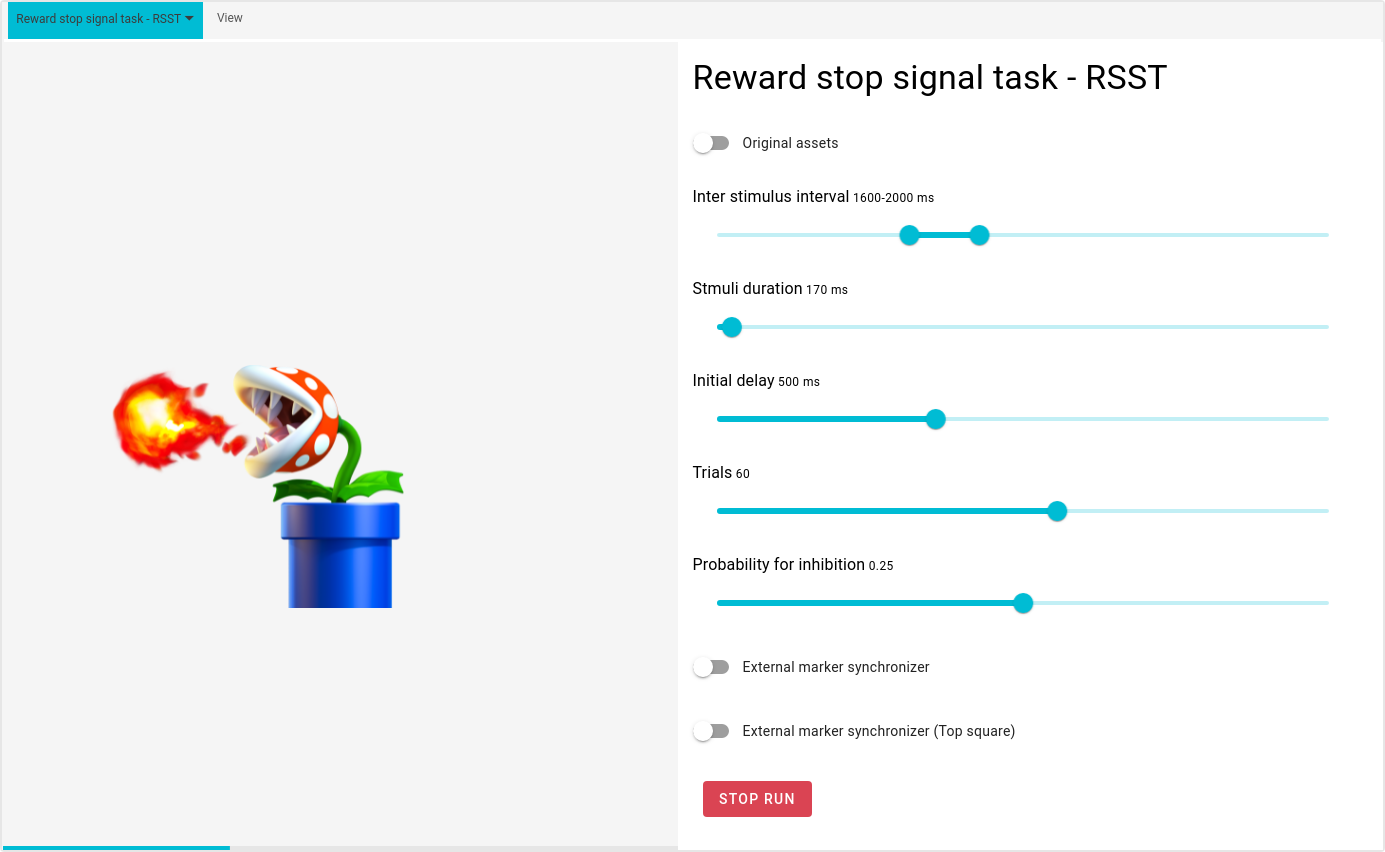
\includegraphics[width=1\textwidth]{Appendix/paradigms/Figures/rsst-delivery.png}
\par\end{centering}
\caption{\gls*{RSST} stimuli delivery dashboard.}
\label{}
\end{figure}